\documentclass{article}

%package setup
\usepackage{graphicx}
\usepackage{amsmath}
\usepackage{fancyhdr}
\usepackage[margin=1in]{geometry}
\usepackage{comment}
\usepackage{placeins}
\usepackage{parskip}
\usepackage{subcaption}
\usepackage{appendix}
\usepackage{soul}
\usepackage{comment}
\usepackage[hidelinks]{hyperref}
\usepackage{matlab-prettifier}
\usepackage{minted}
\usepackage{enumitem}
\usepackage{float}
\usepackage{textcomp, gensymb}
\usepackage{caption}


\pagestyle{fancy}
\fancyhf{} % Clear header/footer settings
\rhead{\thepage} % Page number on the right in the header
\lhead{ASE375 Lab Report 5} % Your lab report title on the left

\begin{document}

\begin{titlepage}
  \centering
  
\includegraphics[width=10cm]{ase-logo-formal.png}  % Adjust the width as needed
  \vspace{1cm}  % Add some vertical space
 
  \Large \textbf{ASE 375 Electromechanical Systems}\\
  \large \textbf{Section 14115}\\
  \vspace{0.5cm}
  \textbf{Monday: 3:00 - 6:00 pm}\\
 
  \vspace{1cm}
 
  \hrule
  \vspace{0.5cm}
 
  \Huge \textbf{Report 6:\\
  Measuring Dynamic Response with Accelerometers}\\
  \Huge \textbf{}\\
 
  \vspace{0.5cm}
  \hrule
 
  \vspace{1cm}
 
  \normalsize \textbf{Andrew Doty, Andres Suniaga, Dennis Hom}\\
  \normalsize \textbf{Due Date: 03/25/2024}
 
\end{titlepage}
\newpage

\tableofcontents
\thispagestyle{empty}
\newpage

\section{Introduction}
This experiment explores the dynamic response of a built-up wing from measurements using (1) a Piezoelectric accelerometer and (2) a Micro-Electro-Mechanical system (MEMS) accelerometer. The goal of this lab experiment is to learn how the accelerometers work by performing a resonance assessment profile (rap or impulse) test on the make-shift wing. 
\vspace{5mm}

The piezoelectric accelerometer cannot measure static quantities, meaning it does not take into the account the force exerted by gravity. On the other hand, the MEMS accelerometer does take into account the gravitational force in its measurements. This lab experiment provides a foundation for understanding the operational aspects of the accelerometers as well as a rap test use-case that show how these sensors are applied in testing of aircraft surfaces.

\section{Equipment}
Measurement devices and hardware used in this lab include:
\begin{itemize}

\item Built-Up Wing Model: 
\vspace{1mm}

In this lab we will use a scaled-down wing model for performing the rap test. This form of experiment is useful in application as rap tests are performed on control surfaces of aircraft.

\begin{figure}[H]
    \centering
    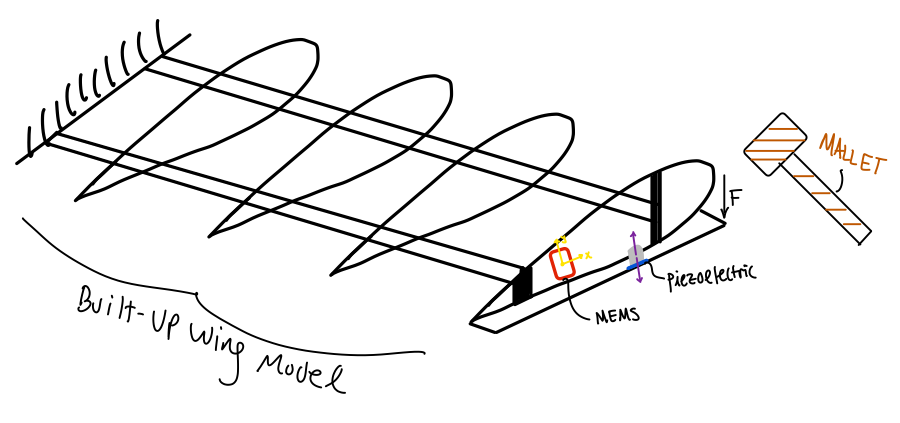
\includegraphics[width = 0.8\textwidth]{lab6images/wingmodellab6.png}
    \caption{Sketch of Built-Up Wing Model setup}
    \label{fig:wingmodel}
\end{figure}
\vspace{2.5mm}

\item Piezoelectric Accelerometer (IMI 660)
\vspace{1mm}

An IMI Series 660 accelerometer is used in the experiment. This Piezoelectric accelerometer only measures acceleration in one direction, and is placed on the built-up wing model as shown in Figure \ref{fig:wingmodel}.\\[1mm]
The operational principle of the Piezoelectric accelerometer is in it piezoelectric crystal, which generates charge from applied stress. It converts mechanical energy into electrical energy. The crystal acts like a capacitor (stores electrical energy). Operational Voltage = $5\text{V}$
\vspace{2.5mm}

\item MEMS Accelerometer (ADXL335)
\vspace{1mm}

The ADXL335 is a small 3-Axis MEMS Accelerometer which operates based on differential capacitance. An applied force or acceleration will change the capacitance within the MEMS accelerometer. In this experiment, the MEMS accelerometer is placed as shown in Figure \ref{fig:wingmodel}, using only the X-and Y-axes. Operational Voltage = $3.3\text{V}$
\vspace{2.5mm}

\item Brass Mallet: 
\vspace{1mm}

A brass mallet is used to apply a tap force to the built-up wing model as shown in Figure \ref{fig:wingmodel}. 
\vspace{2.5mm}

\item DAQ, NI-9215 Voltage Input Module, and LabVIEW:
\vspace{1mm}

Data Acquisition System used to process sample measurements into digital data. NI-9215 is an analog input module used to measure the output voltage signals of sensors and send it through the DAQ system. LabVIEW used to model these output voltages read from the DAQ of the accelerometer measurements. We connect to the $3.3 \text{V}$ and $5 \text{V}$ ports of the DAQ for our experiment.
\vspace{2.5mm}

\item Solderless Breadboard, Jumper Wires: 
\vspace{1mm}

Used to make connections to the input analog modules and to construct circuits. In this lab we connect the accelerometer inputs to the breadboard for power, ground, and signal to the measurement axes.

\end{itemize}

\section{Procedure}
Before beginning the experiment, we must build the block diagram which will be executed by LabVIEW to gather our accelerometer measurements. 

\begin{figure}[H]
    \centering
    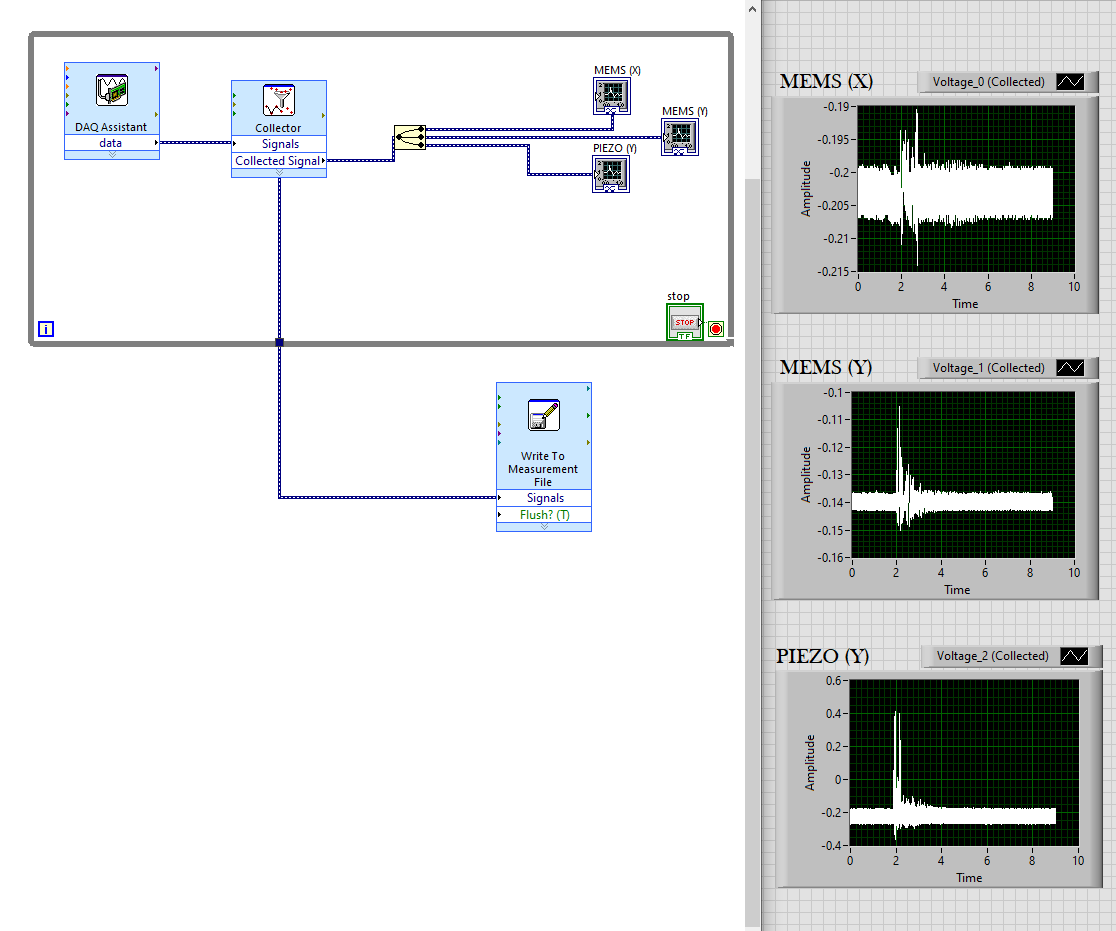
\includegraphics[width = 0.75\textwidth]{lab6images/blockdiagramlab6.PNG}
    \caption{LabVIEW Model Setup for Accelerometers}
    \label{fig:labview}
\end{figure}

\subsection{Accelerometer Setup and Experiment}
\begin{enumerate}
    \item  First, connect the MEMS and Piezoelectric accelerometers accordingly to power and ground, and connect the signal wires to corresponding NI-9215 ports. 
    \item Place the MEMS and Piezoelectric accelerometer on the wing model as shown in Figure \ref{fig:wingmodel}.
    \item Before hitting the wing with the brass mallet, the test that the MEMS and Piezoelectric accelerometers work by applying a force and observing the corresponding output in LabVIEW. Continue to the next step once working. If not working, check possible issues which may include:
    \begin{itemize}
        \item Connections on breadboard
        \item Faulty wires from NI-9215 Port
        \item Faulty accelerometer sensor
    \end{itemize}
    \item Run the LabVIEW model as shown in Figure \ref{fig:labview} and tap the wing with the brass mallet. Let it record the accelerometer data for 5 seconds. Save the data to a file and ensure it has been written correctly.
    \item Repeat previous step (3) for 10 measurements. 
    \item Once complete, we are ready to plot the measured accelerations and evaluate the data. From this we can identify the natural frequencies of the wing.
\end{enumerate}

\hypertarget{datapro}{}
\section{Data Processing}
% \subsection{Variables and Equations}  

% Newton's 2nd Law:

% \begin{equation}
%     a = \dfrac{F}{m}
% \end{equation}

% Variables:
% \begin{enumerate}[label = \Roman*.]
%     \item \( V \): Voltage
% \end{enumerate}

\subsection{Script Pseudocode}

For the accelerometer portion of the lab, prior to the power spectrum analysis, all calculations were finished using this \textsc{Matlab} script. The pseudocode is here, and the full \textsc{Matlab} code will be detailed in the appendix \ref{accscript}.

\begin{minted}[breaklines, linenos]{yaml}
    read_data:
      file_path: "Lab Data/Lab6__1.xlsx"
    
    processing_steps:
      - read_table: 
          input: "Lab Data/Lab6__1.xlsx"
      - generate_time_sequence:
          start: 0.001
          end: 10
          step: 0.001
      - select_data_columns:
          columns: [2, 4, 6]
      - convert_to_array:
          input: data
      - calculate_averages:
          axis: 1
      - normalization:
          subtract: averages
          adjust_for_calibration:
            - mems_x: "scale by CaliMems"
            - mems_y: "scale by CaliMems, convert to degrees"
            - piezo_y: "scale by CaliPiezo, adjust scale factor"
      - fft_analysis:
          components: [X, mems_x, mems_y]
      - numerical_integration:
          calculate_velocity_and_displacement: true
      - plot_data:
          figures:
            - figure_1: "Acceleration and Velocity plots"
            - figure_2: "Displacement plots"
            - figure_3: "Frequency Response Analysis"
    
    calibration_constants:
      CaliMems: "300*3.3/3, converted to V/(m/s^2)"
      CaliPiezo: "10, converted to V/(m/s^2)"
    
    analysis:
      frequency_response:
        initial_analysis:
          period: "5 seconds"
        follow_up_analysis:
          period: "last second"
      derive_natural_frequencies:
        method: "find peak amplitude locations"
      compile_results:
        format: table
        contents: "Sensor, Frequency at 5 seconds, Frequency at Last Second"
\end{minted}

For the power spectrum analysis, the following script was used in psuedocode and will be detailed in the appendix \ref{powerspec}.

\begin{minted}[breaklines, linenos]{yaml}
    file_processing:
      directory_path: "Lab Data/*.xlsx"
      get_files_and_folders: true
      file_check: 
        is_file: true
    
    initializations:
      figure: 1
      natural_frequencies_5_seconds: []
      natural_frequencies_last_second: []
    
    processing_steps:
      for_each_file:
        if: "is_file"
        operations:
          - read_file:
              path: "Full path based on directory and file name"
              action: "Read table from Excel file"
          - preprocess_data:
              time_sequence: "0.001 to 10 in 0.001 increments"
              select_columns: [2, 4, 6]
              convert_to_array: true
              calculate_averages: true
              normalize_data: "Subtract averages, adjust for CaliPiezo"
          - fft_analysis:
              component: "data_norm(:,3)"
              frequency_range: "0 to 1000"
              calculate_amplitude: true
          - plot_frequency_response:
              figure: 1
              plot: "Frequency vs. Amplitude (5 seconds)"
              title: "Piezo (5 seconds)"
              add_legend: true
          - identify_natural_frequency:
              find_maximum_amplitude_location: true
              store_frequency: "NaturalFreqV0_5"
          - optional_section:
              commented_out: true
              description: "Analysis for the last second is prepared but not executed"
    
    second_loop:
      description: "Repeat steps for second analysis focusing on the last second"
      operations:
        - adjust_data_set: "Halve N, adjust frequency range"
        - fft_analysis:
            component: "data_norm(:,3) for last half"
            calculate_amplitude: true
        - plot_frequency_response:
            figure: 2
            plot: "Frequency vs. Amplitude (Last second)"
            title: "Piezo (Last second)"
            add_legend: true
        - identify_natural_frequency:
            find_maximum_amplitude_location: true
            store_frequency: "NaturalFreq_LastSec"
    
    final_steps:
      remove_initial_zeros: "NaturalFreq_LastSec adjustment"
      calculate_averages:
        - average_frequency_5_seconds: "Mean of NaturalFreqV0_5"
        - average_frequency_last_second: "Mean of NaturalFreq_LastSec"
\end{minted}

The above power spectrum analysis script processes acceleration data from Excel files, normalizing and calibrating it before applying a Fast Fourier Transform (FFT) to shift from time domain to frequency domain. This reveals the power distribution across frequencies, allowing for identification of dominant frequencies or natural vibrations. It calculates the mean amplitudes over two distinct time intervals to detect any shifts in vibration characteristics, providing critical insights into the dynamic response of the system under observation.
    
\section{Results and Analysis}

\subsection{Accelerometer Data}

The piezoelectric data and MEMS accelerometer data were collected and analyzed in LabVIEW. The data was collected for 10 seconds in each iteration instead of 5 so that way the effects of the perturbation have more time to level out. The data collected is shown in Figure \ref{fig:disvelaccdata}.



\begin{figure}[H]
    \centering
    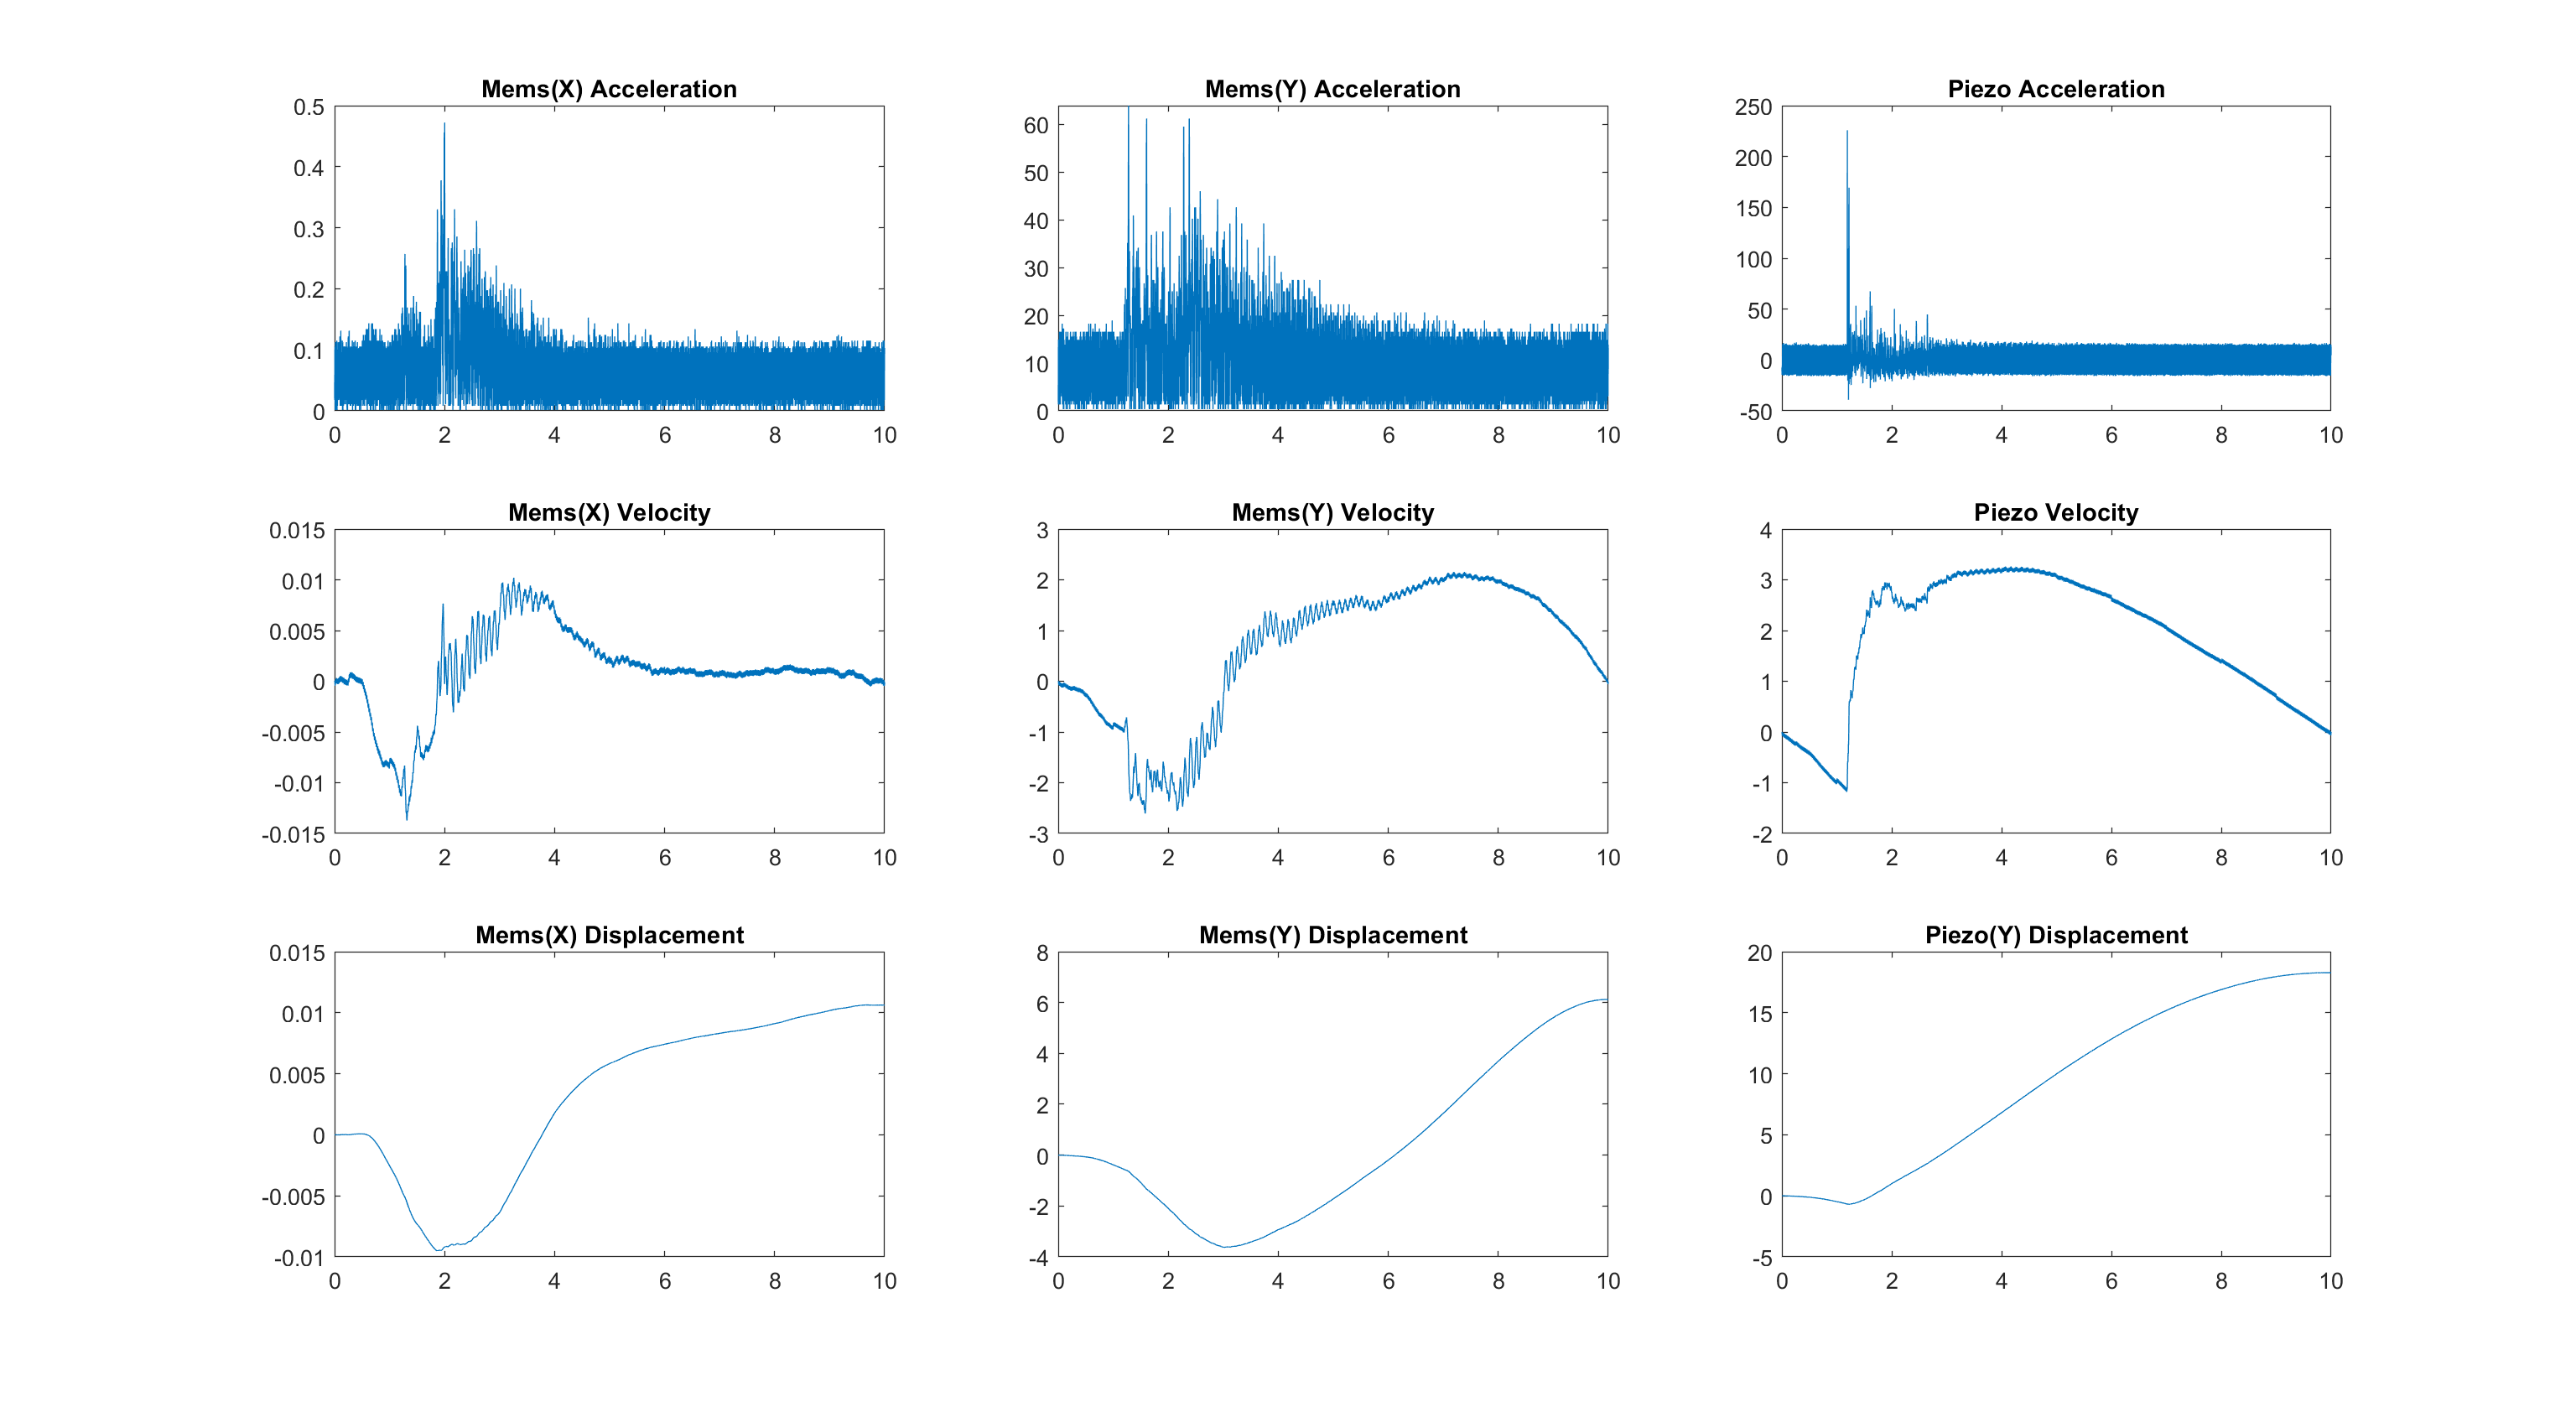
\includegraphics[width = 1\textwidth]{lab6images/disvelaccdata.png}
    \caption{Acceleration, Velocity, and Displacement Data}
    \label{fig:disvelaccdata}
\end{figure}

In the graphs, we can clearly see the acceleration present from the initial disturbance, a velocity profile indicative of the acceleration, and a displacement profile indicative of the velocity. However, although these graphs are useful for understanding the data, there are errors inherent in the data that need to be addressed. The data is noisy and has a lot of high-frequency noise that needs to be filtered out, which can clearly be seen in the acceleration data. That band of noise is quite wide, for X acceleration the noise band is 0.1 with a peak acceleration near 0.5, and for Y acceleration the noise band is around 15 with a peak acceleration near 60. Lastly, the Piezo data shows a noise band of around 40 with a peak near 240. While the noise is also present in the velocity and displacement data, it is not as pronounced as in the acceleration data due to the integration process to get those results. However, that does not mean that the noise is not present in the velocity and displacement data, the integration is including it in the measurements and distorting the results. To have a higher power signal-to-noise ratio, we need to filter out the noise in the data. We accomplished that using a power spectrum analysis in \textsc{Matlab}.

\subsection{Power Spectrum Analysis}

The power spectrum analysis should help filter out the noise in the data and identify the natural frequency. This was accomplished using the script whose pseudocode was detailed in the previous section. The results of the power spectrum analysis are shown in Figures \ref{fig:freqresponse5} and \ref{fig:freqresponselast}.

\begin{figure}[H]
    \centering
    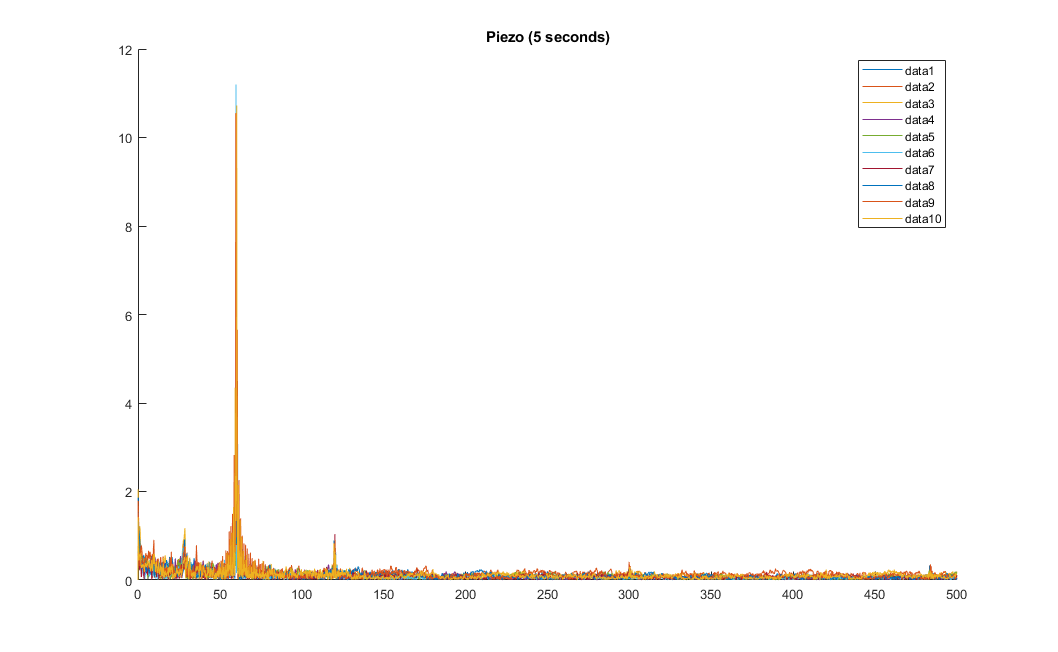
\includegraphics[width = 0.8\textwidth]{lab6images/frequencyanalysis5second.png}
    \caption{Frequency Analysis 5 Seconds}
    \label{fig:freqresponse5}
\end{figure}

\begin{figure}[H]
    \centering
    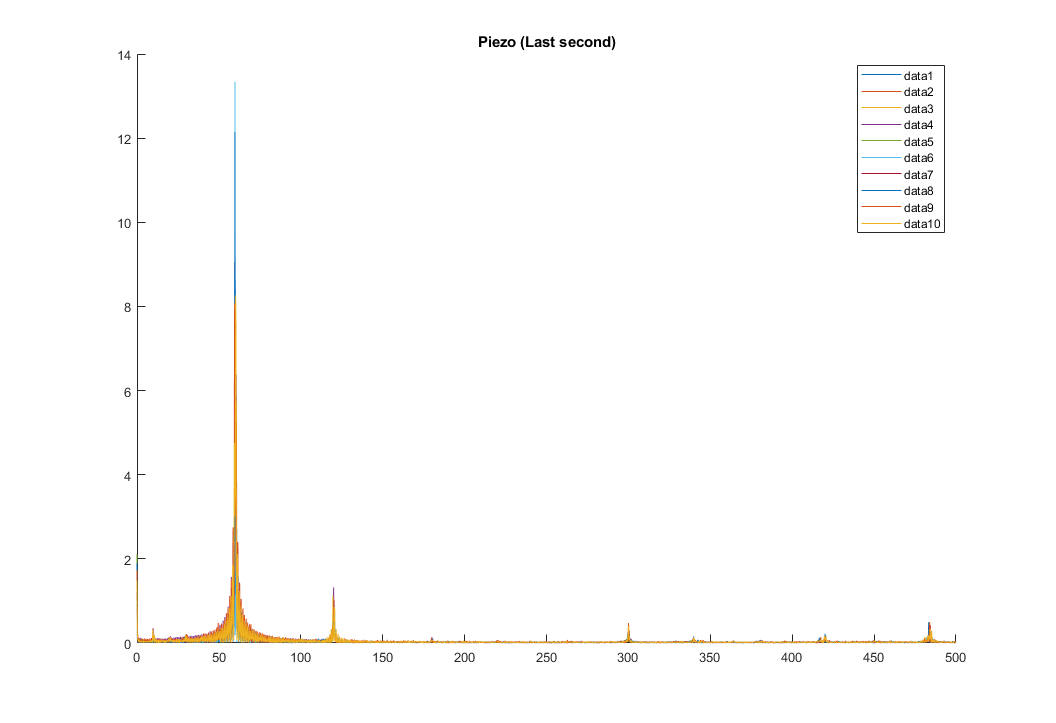
\includegraphics[width = 0.8\textwidth]{lab6images/frequencyanalysislastsecond.png}
    \caption{Frequency Analysis Last Second}
    \label{fig:freqresponselast}
\end{figure}

This frequency response shows the noise present at higher frequencies in the oscillations, but a very dominant natural frequency appears at around 59.9 Hz in all cases, despite variations in the noise below the natural frequency and above the natural frequency. Computing the specific natural frequency for each case numerically, we get:

Natural Frequency 5 seconds = \\
\(\left[59.9060,\,   60.2289,\,   59.8060,\,   59.7060,\,  59.8060,\,   59.8060,\,   59.7060,\,   59.7844,\,   59.6733,\,   60.3060\right]\)

Natural Frequency Last Second = \\
\(\left[60.0120,\,   59.7911,\,   59.8120,\,   59.6119,\,  59.8120,\,   59.8120,\,   59.8120,\,   59.7911,\,   59.5688,\,   60.2120\right]\)

Average Natural Frequency over 5 Seconds = 59.8729  % The average frequency calculated over a 5-second time interval.

Average Natural Frequency over Last Second = 59.8235  % The average frequency calculated over the last second of the data.

The very close alignment between the natural frequencies highlights the accuracy of our approach. In addition, the average natural frequency over the 5-second interval is very close to the average natural frequency over the last second, indicating the stability of the system's dynamic response. This power spectrum analysis enables us to use various filters to remove noise now that we have identified the natural frequency of the system.

\section{Conclusion}
In this lab experiment we learned how the piezoelectric and MEMS accelerometers operate in order to measure acceleration and perform frequency analysis of an aircraft surface. These devices are very practical in analyzing aircraft control surfaces that experience lots of vibration as these sensors are very responsive to forces. Analysis of these surfaces provides critical information useful to the structural dynamics of an aircraft. Due to this, accelerometers play an important role in ensuring an aircraft is safe to fly, and power spectrum analysis allows for the identification of natural frequencies of the system. The results of the power spectrum analysis show that the natural frequency of the system is around 59.9 Hz, which is very close to the average natural frequency over the last second of the data. This indicates that the system is stable and has a consistent dynamic response.

\newpage
\thispagestyle{empty}  % Clear header/footer
\begin{center}
	\vspace*{\fill}
	{\Huge Appendix}
	\vspace*{\fill}
\end{center}

% Start appendices
\newpage
\begin{appendices}
\pagestyle{fancy}
\renewcommand{\thefigure}{A\arabic{figure}}
\setcounter{figure}{0}

% \section*{t-Distribution Tables}
% \hypertarget{1}{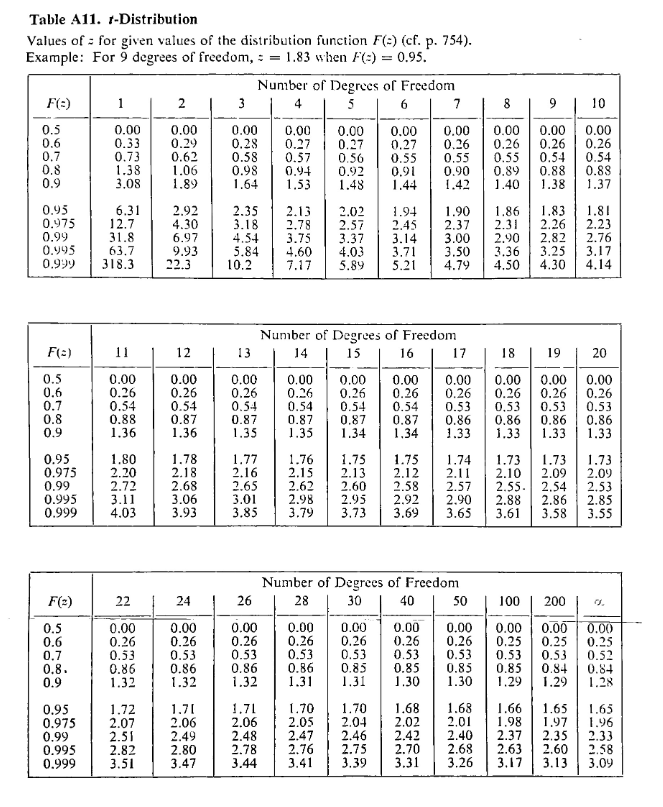
\includegraphics[width=0.95\textwidth]{t_distribution_Table_lecture3.png}}

\newpage

\section*{Accelerometer Analysis \textsc{Matlab} Script}
\label{accscript}
\begin{minted}[breaklines, linenos]{matlab}
    T=readtable("Lab Data/Lab6__1.xlsx");

    time=0.001:0.001:10;
    data=[T(:,2) T(:,4) T(:,6)];
    data=table2array(data);
    averages=mean(data,1);
    [N,M]=size(T);
    % 1:mems (x)
    % 2:mems (y)
    % 3:piezo (y)
    CaliMems=300*3.3/3; %mv/g
    CaliMems=CaliMems*1/1000/9.81; %V/(m/s^2)
    CaliPiezo=10; %mV/g
    CaliPiezo=CaliPiezo*1/1000/9.81; %V/(m/s^2)
    data_norm=bsxfun(@minus, data , averages);
    data_norm(:,3)=data_norm(:,3)/CaliPiezo/2.815;
    data_norm(:,1)=data_norm(:,1)/CaliMems; %mems x
    data_norm(:,2)=data_norm(:,2)/CaliMems*180; %mems y
    X=data_norm(:,3);
    
    
    V0=fft(data_norm(:,1));
    V1=fft(data_norm(:,2));
    V2=fft(data_norm(:,3));
    Frequency=linspace(0,1000,N);
    
    %Numerical Integration
    VelMemX=cumtrapz(time,data_norm(:,1));
    VelMemX=VelMemX-VelMemX(1);
    VelMemY=cumtrapz(time,data_norm(:,2));
    VelMemY=VelMemY-VelMemY(1);
    VelPiezoY=cumtrapz(time,X);
    VelPiezoY=VelPiezoY-VelPiezoY(1);
    disMemX=cumtrapz(time,VelMemX);
    disMemX=disMemX-disMemX(1);
    disMemY=cumtrapz(time,VelMemY);
    disMemY=disMemY-disMemY(1);
    disPiezoY=cumtrapz(time,VelPiezoY);
    disPiezoY=disPiezoY-disPiezoY(1);
    
    figure(1)
    subplot(3,3,1)
    plot(time,abs(data_norm(:,1)))
    title('Mems(X) Acceleration')
    subplot(3,3,2)
    plot(time,abs(data_norm(:,2)))
    title('Mems(Y) Acceleration')
    subplot(3,3,3)
    plot(time,X)
    title('Piezo Acceleration')
    
    subplot(3,3,4)
    plot(time,VelMemX)
    title('Mems(X) Velocity')
    subplot(3,3,5)
    plot(time,VelMemY)
    title('Mems(Y) Velocity')
    subplot(3,3,6)
    plot(time,VelPiezoY)
    title('Piezo Velocity')
    subplot(3,3,7)
    plot(time,disMemX)
    title('Mems(X) Displacement')
    subplot(3,3,8)
    plot(time,disMemY)
    title('Mems(Y) Displacement')
    subplot(3,3,9)
    plot(time,disPiezoY)
    title('Piezo(Y) Displacement')
    
    
    %Frequency Response
    
    Amplitude1=2/N*real(abs(V0));
    Amplitude2=2/N*real(abs(V1));
    Amplitude3=2/N*real(abs(V2));
    % 5 Seconds
    figure(2);
    subplot(3,2,1)
    plot(Frequency(1:N/2),Amplitude1(1:N/2))
    title('Mems(X) (5 seconds)')
    subplot(3,2,3)
    plot(Frequency(1:N/2),Amplitude2(1:N/2))
    title('Mems(Y) (5 seconds)')
    subplot(3,2,5)
    plot(Frequency(1:N/2),Amplitude3(1:N/2))
    title('Piezo (5 seconds)')
    
    loc1=Amplitude1==max(Amplitude1(1:N/2));
    loc2=Amplitude2==max(Amplitude2(1:N/2));
    loc3=Amplitude3==max(Amplitude3(1:N/2));
    
    NaturalFreqV0=Frequency(loc1);
    NaturalFreqV1=Frequency(loc2);
    NaturalFreqV2=Frequency(loc3);
    
    NaturalFreqV0_5=NaturalFreqV0(1);
    NaturalFreqV1_5=NaturalFreqV1(1);
    NaturalFreqV2_5=NaturalFreqV2(1);
    % Last second
    N2=N2/2;
    Frequency=linspace(0,1000,N2);
    data_norm(1:N2,:)=[];
    V0=fft(data_norm(:,1));
    V1=fft(data_norm(:,2));
    V2=fft(data_norm(:,3));
    Amplitude1=2/N2*real(abs(V0));
    Amplitude2=2/N2*real(abs(V1));
    Amplitude3=2/N2*real(abs(V2));
    
    subplot(3,2,2)
    plot(Frequency(1:N2/2),Amplitude1(1:N2/2))
    title('Mems(X) (Last second)')
    subplot(3,2,4)
    plot(Frequency(1:N2/2),Amplitude2(1:N2/2))
    title('Mems(Y) (Last second)')
    subplot(3,2,6)
    plot(Frequency(1:N2/2),Amplitude3(1:N2/2))
    title('Piezo (Last second)')
    
    loc1=find(Amplitude1==max(Amplitude1(1:N2/2)));
    loc2=find(Amplitude2==max(Amplitude2(1:N2/2)));
    loc3=find(Amplitude3==max(Amplitude3(1:N2/2)));
    
    NaturalFreqV0=Frequency(loc1);
    
    NaturalFreqV1=Frequency(loc2);
    NaturalFreqV2=Frequency(loc3);
    
    NaturalFreqV0_Last=NaturalFreqV0(1);
    NaturalFreqV1_Last=NaturalFreqV1(1);
    NaturalFreqV2_Last=NaturalFreqV2(1);
    
    Frequency_5s=[NaturalFreqV0_5; NaturalFreqV1_5; NaturalFreqV2_5];
    Frequency_LastSec=[NaturalFreqV0_Last; NaturalFreqV1_Last; NaturalFreqV2_Last];
    Sensor=["Mems(X)";"Mems(Y)";"Piezo(Y)"];
    Table=table(Sensor, Frequency_5s, Frequency_LastSec)
\end{minted}

\section*{Power Spectrum Analysis \textsc{Matlab} Script}
\label{powerspec}
\begin{minted}[breaklines, linenos]{matlab}
    % Get a list of all files and folders in the directory
    Files = dir('Lab Data/*.xlsx');
    i=1;
    % Get a logical vector that tells which is a file
    isFile = ~[Files.isdir];
    figure()
    % Loop only over the files
    for iExcelSubject = 1:length(Files)
        if isFile(iExcelSubject)
            % Full path to file
            Report = fullfile('Lab Data', Files(iExcelSubject).name);
            % Read the table from the Excel file
            T = readtable(Report);
            % Do something with table T
            % ...
            time=0.001:0.001:10;
    data=[T(:,2) T(:,4) T(:,6)];
    data=table2array(data);
    averages=mean(data,1);
    [N,M]=size(T);
    % 1:mems (x)
    % 2:mems (y)
    % 3:piezo (y)
    CaliPiezo=10; %mV/g
    CaliPiezo=CaliPiezo*1/1000/9.81; %V/(m/s^2)
    data_norm=bsxfun(@minus, data , averages);
    data_norm(:,3)=data_norm(:,3)/CaliPiezo/2.815;


    V0=fft(data_norm(:,3));
    Frequency=linspace(0,1000,N);
    Amplitude1=2/N*real(abs(V0));
    hold on;
    figure(1)
    plot(Frequency(1:N/2),Amplitude1(1:N/2))
    title('Piezo (5 seconds)')
    legend()

    loc1=Amplitude1==max(Amplitude1(1:N/2));
    NaturalFreqV0=Frequency(loc1);
    NaturalFreqV0_5(i)=NaturalFreqV0(1);

    i=i+1;
    % N2=N/2;
    % Frequency=linspace(0,1000,N2);
    % data_norm(1:N2,:)=[];
    % V0=fft(data_norm(:,1));
    % Amplitude1=2/N2*real(abs(V0));
    % hold on;
    % figure(2)
    % plot(Frequency(1:N2/2),Amplitude2(1:N2/2))
    % title('Piezo (Last second)')
    % legend()
        end
    end
    hold off;


    figure();
    hold on;
    % Loop only over the files
    for iExcelSubject = 1:length(Files)
        if isFile(iExcelSubject)
            % Full path to file
            Report = fullfile('Lab Data', Files(iExcelSubject).name);
            % Read the table from the Excel file
            T = readtable(Report);
            % Do something with table T
            % ...
            time=0.001:0.001:10;
    data=[T(:,2) T(:,4) T(:,6)];
    data=table2array(data);
    averages=mean(data,1);
    [N,M]=size(T);
    % 1:mems (x)
    % 2:mems (y)
    % 3:piezo (y)
    CaliPiezo=10; %mV/g
    CaliPiezo=CaliPiezo*1/1000/9.81; %V/(m/s^2)
    data_norm=bsxfun(@minus, data , averages);
    data_norm(:,3)=data_norm(:,3)/CaliPiezo/2.815;


    % V0=fft(data_norm(:,3));
    % Frequency=linspace(0,1000,N);
    % Amplitude1=2/N*real(abs(V0));
    % hold on;
    % figure(1)
    % plot(Frequency(1:N/2),Amplitude1(1:N/2))
    % title('Piezo (5 seconds)')
    % legend()

    N2=N/2;
    Frequency=linspace(0,1000,N2);
    data_norm(1:N2,:)=[];
    V0=fft(data_norm(:,3));
    Amplitude1=2/N2*real(abs(V0));
    hold on;
    figure(2)
    plot(Frequency(1:N2/2),Amplitude1(1:N2/2))
    title('Piezo (Last second)')
    legend()

    loc1=Amplitude1==max(Amplitude1(1:N2/2));
    NaturalFreqV0=Frequency(loc1);
    NaturalFreq_LastSec(i)=NaturalFreqV0(1);

    i=i+1;
        end
    end
    hold off;

    NaturalFreqV0_5
    NaturalFreq_LastSec;
    NaturalFreq_LastSec=NaturalFreq_LastSec(11:end)
    Avg5SecFreq=mean(NaturalFreqV0_5)
    AvgLastSecFreq=mean(NaturalFreq_LastSec)

\end{minted}

\section*{NI-9215 Datasheet}
\url{https://www.amc-systeme.de/files/pdf/ni-9215-amc.pdf}

\section*{IMI Series 660 Accelerometer Datasheet}
\url{https://pim-kft.hu/wp-content/uploads/2016/02/PCB_LowCost_Embeddable_Accelerometers.pdf}

\section*{ADXL335 Accelerometer Datasheet}
\url{https://www.analog.com/media/en/technical-documentation/data-sheets/adxl335.pdf}

\end{appendices}

\end{document}
